\documentclass{article}
\usepackage{graphicx} % Required for inserting images
\usepackage{authblk}
\usepackage{cite}
\usepackage{natbib}
\usepackage{dcolumn}
\usepackage{pdfpages}
\usepackage{epigraph} % Required for inspirational quote
% packages required for kable()
\usepackage{booktabs}
\usepackage{longtable}
\usepackage{array}
\usepackage{multirow}
\usepackage{wrapfig}
\usepackage{float}
\usepackage{colortbl}
\usepackage{pdflscape}
\usepackage{tabu}
\usepackage{threeparttable}
\usepackage{threeparttablex}
\usepackage[normalem]{ulem}
\usepackage{makecell}
\usepackage{xcolor}
\renewcommand{\epigraphsize}{\small}
\setlength{\epigraphwidth}{0.51\textwidth}
\renewcommand{\textflush}{flushright}
\renewcommand{\sourceflush}{flushright}

% display code
\usepackage{listings}
\usepackage{color}

\definecolor{dkgreen}{rgb}{0,0.6,0}
\definecolor{gray}{rgb}{0.5,0.5,0.5}
\definecolor{mauve}{rgb}{0.58,0,0.82}
\lstset{frame=tb,
  language=Java,
  aboveskip=3mm,
  belowskip=3mm,
  showstringspaces=false,
  columns=flexible,
  basicstyle={\small\ttfamily},
  numbers=none,
  numberstyle=\tiny\color{gray},
  keywordstyle=\color{blue},
  commentstyle=\color{dkgreen},
  stringstyle=\color{mauve},
  breaklines=true,
  breakatwhitespace=true,
  tabsize=3
}


%\date{Draft -- please do not circulate.}

\title{SEM: Research Questions}

\author[1]{David Broska}

\begin{document}
\maketitle

\section{Intro}

In my submission for the multilevel modeling research project, I found that liberals/Democrats perceive online comments on average as more toxic than conservatives/Republicans. \textit{What explains differences in perceived toxicity in conversations between liberals and conservatives?} Below, I will break this question down into subquestions and describe the data I plan to use for the mediation analyses.


On the individual level, I use mediation analysis to investigate the psychological processes related to why liberals perceive content as more toxic. \textit{Do liberals learn to perceive content as toxic?} If not, political ideology represents an independent effect.

\begin{itemize}
    \item It may be the case that education trains individuals to be more sensitive toward issues, and liberals are more educated on average than conservatives. Hence, higher levels of education mediate higher perceived toxicity. 
    \item What has been considered a peccadillo by older cohorts is now a major transgression in the eyes of younger individuals, and conservatives are on average older than liberals. Hence, higher age is associated with lower perceived toxicity. 
\end{itemize}


\textit{Do liberals perceive content as more toxic because they see different forms of engagement?}

\begin{itemize}
    \item Liberals see more toxicity because they see less rational engagement in conversations than conservatives. In other words, liberals may have higher standards for a deliberative dialogue, and perceiving less of these deliberative forms of communication explains their higher toxicity ratings. This involves seeing less openness, less objectivity, less effort, more emotional engagement, and more transgressions from the topic of the conversations.
    \item Liberals see more toxicity because they see less polite forms of engagement in conversations than conservatives, explaining why they see more toxicity. This involves perceiving less respectful engagement, more sarcasm, more hostility, and less tolerance. 
\end{itemize}

There are interesting implications here. It may that liberals mostly care about politeness. This happens if forms of rational engagement do not mediate the association between political ideology and perceived toxicity but politeness does. 



\section{Data}

I will use the same data as for my multilevel modeling study. To study the determinants of perceived civility in conversations, we recruit 4,675 American adults via Prolific to fill out a survey asking them to evaluate Facebook conversations regarding perceived toxicity and other features. Respondents who did not pass an attention check were not allowed to take the survey. Excluding missing values, the total sample size is 32,597 observations. Those who passed the attention check were randomly assigned to evaluate 7 conversations. Not every respondent evaluated each conversation; each one was evaluated 3.27 times on average. These data are for addressing the questions outlined above because we measured several outcome variable tapping into a broad range of perceptions of conversations (see Figure below for a plot of the variables). 

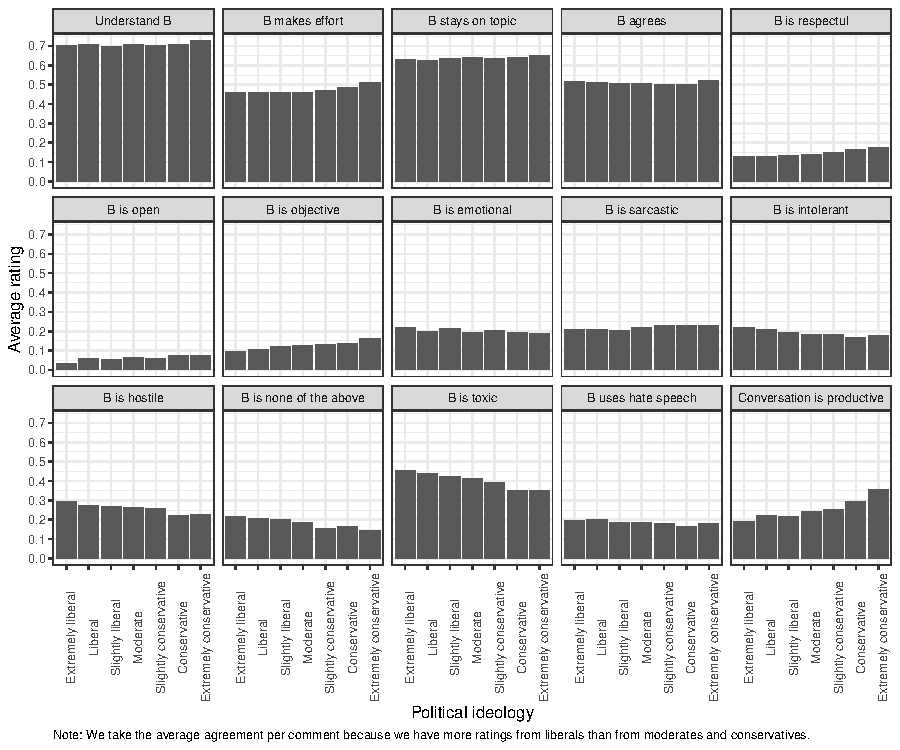
\includegraphics[]{figures/2_AvgAgreement_Ideo.pdf}

\end{document}


% individual
% topic 
% topic, 
% different 
% turn-taking
% topic 
% length mirroring
% range of words
% negativity, positivity
% content vs form 
% uptake of conversations 
% Liberals are numb to conversational moves
% A short introduction Habermas Oxford University green
% cultural mindset (everything is agency, everything inequality)
% do conservatives see the whole conservation, and liberals just the particular-- whos attenued to the conversation
% we view disagreement the same way (punchy, disagreement, range of words net of length = intellectual ) 
% limit to short or long